\section{Package}
\label{sec:Package}
Grundsätzlich ist ein Package eine Ansammlung von mehreren Quests. Dadurch soll es den Erstellern von Quests ermöglicht werden, die Aufgaben in Bereiche zu gliedern. Programmtechnisch bilden mehrere Quests, welche in einem Ordner zusammengefasst werden, ein Package.

\subsection{Organisation von Packages und Quests}
\begin{figure}[h] 
  \centering
     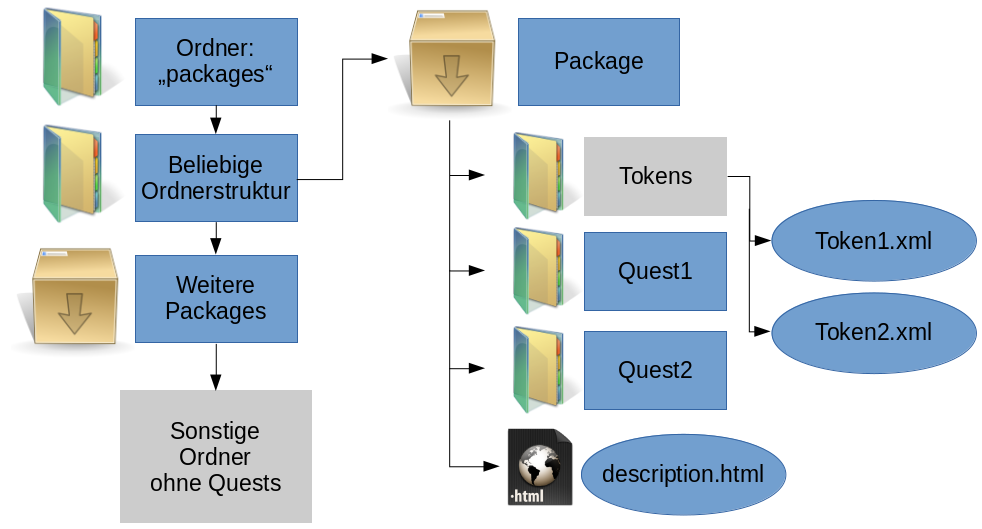
\includegraphics[width=0.8\textwidth]{./media/images/quest/ordnerstruktur.png}
  \caption{Beispielhafte Darstellung einer Ordnerstruktur}
  \label{fig:package_ordnerstruktur_1}
\end{figure}
Wie aus der Abbildung \ref{fig:package_ordnerstruktur_1} erkennbar ist, können Packages in beliebigen Ordnerstrukturen organisiert sein. Sobald ein Ordner auftritt, welcher keine Quest beinhaltet, wird dieser von der Auswahl ausgeschlossen. Es können auch übergeordnete Packages erstellt werden. Dies hat vor allem Sinn, wenn Packete wiederum in mehrere Kapitel unterteilt werden sollen.

Ein Ordner in der Package-Auswahl kann auch wie eine Quest eine Beschreibung “\textbf{description.html}”, und ein “\textbf{style.css}” beinhalten.

Im Programm werden die Packages und Quests automatisch anhand des Ordnernamens aufsteigend sortiert. Somit ist es für Ersteller von Packages einfach, diese in die gewünschte Reihenfolge zu bringen.